\textbf{LeVeque 2.1} 

a) Write out the $5 \times 5$ matrix $A$ from (2.43) for the boundary value problem \linebreak $u''(x) = f(x)$ with 
   $u(0) = u(1) = 0$ with a step size of $h = 0.25$.

\begin{solution}\ \\\\
    With a step size of $h = 0.25$, our discretization yields five points and hence our discretization matrix $A$ is 
    given by:

    \begin{align*}
        A &= \frac{1}{h^2}
        \begin{pmatrix}
         h^2 &  0 &  0 &  0 &   0 \\
           1 & -2 &  1 &  0 &   0 \\
           0 &  1 & -2 &  1 &   0 \\
           0 &  0 &  1 & -2 &   1 \\
           0 &  0 &  0 &  0 & h^2 \\
        \end{pmatrix} \\\\
        &= 
        \begin{pmatrix}
             1 &   0 &   0  &   0 &  0 \\
            16 & -32 &  16  &   0 &  0 \\
             0 &  16 & -32  &  16 &  0 \\
             0 &   0 &  16  & -32 & 16 \\
             0 &   0 &   0  &   0 &  1 \\
        \end{pmatrix}.
    \end{align*}
\end{solution}

\pagebreak
b) Write out the $5 \times 5$ inverse matrix $A^{-1}$ explicitly for this problem.

\begin{solution}\ \\\\
    The inverse discretization matrix $A^{-1}$ is given by\footnote{Calculated with MATLAB}:

    \begingroup
    \renewcommand*{\arraystretch}{1.5}
    \begin{align*}
        A^{-1} &=
        \begin{pmatrix}
                      1 &             0 &             0  &             0 &           0 \\
            \frac{3}{4} & -\frac{3}{64} & -\frac{1}{32}  & -\frac{1}{64} & \frac{1}{4} \\
            \frac{1}{2} & -\frac{1}{32} & -\frac{1}{16}  & -\frac{1}{32} & \frac{1}{2} \\
            \frac{1}{4} & -\frac{1}{64} & -\frac{1}{32}  & -\frac{3}{64} & \frac{3}{4} \\
                      0 &             0 &             0  &             0 &           1 \\
        \end{pmatrix}.
    \end{align*}
    \endgroup
\end{solution}

\pagebreak
c) If $f(x) = x$, determine the discrete approximation to the solution of the boundary value problem on this grid and
   sketch this solution and the five Green's functions whose sum gives this solution.


\begin{solution}\ \\\\
    By (2.49) in the text, our discrete approximation to the solution of the boundary problem on a uniform grid with 
    mesh size $h=0.25$ with Dirichlet boundary conditions (i.e., $f(0) = \alpha$ and $f(1) = \beta$) is given by:

    \begin{align*}
        U_i = \alpha (1 - x_i)  + \beta x_i + h \sum\limits_{k=1}^{3}{f(x_k) G(x_i; x_k)}.
    \end{align*}

    where each Green's function $G(x; x_k)$ is given by:

    \begin{align*}
        G(x; x_k) = \begin{cases}
            x(x_k - 1), \text{ for } 0 \le x \le x_k \\
            x_k(x - 1), \text{ for } x_k \le x \le 1 \\
        \end{cases}\, .
    \end{align*}

    The resulting solution and constituent Green's functions are shown below:

    \begin{figure}[h]
        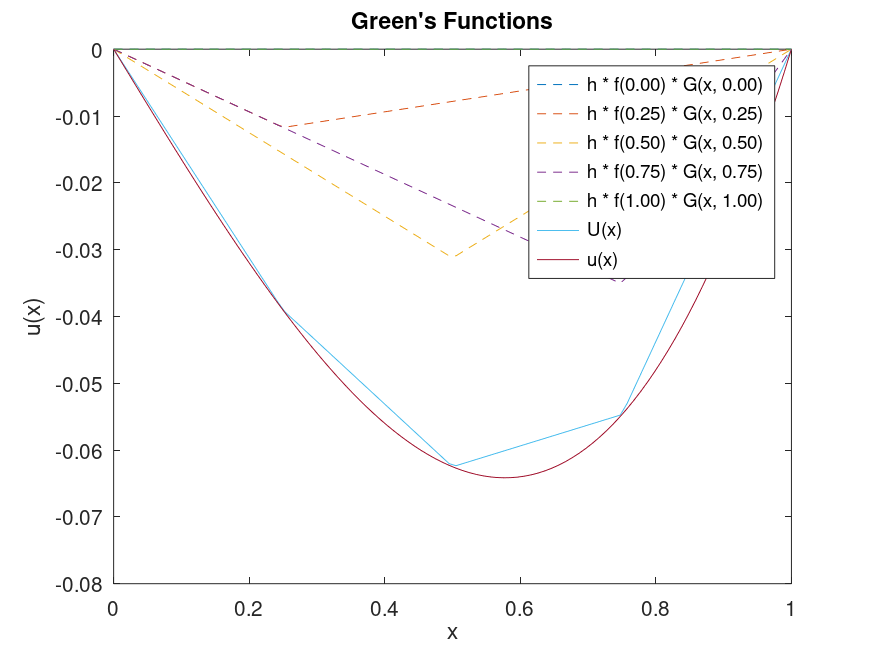
\includegraphics[width=13cm]{problem1c_discrete_approx.png}
        \centering
        \caption{Discrete approximation to $u''(x)=x$ with Dirichlet boundary conditions}
    \end{figure}


\end{solution}